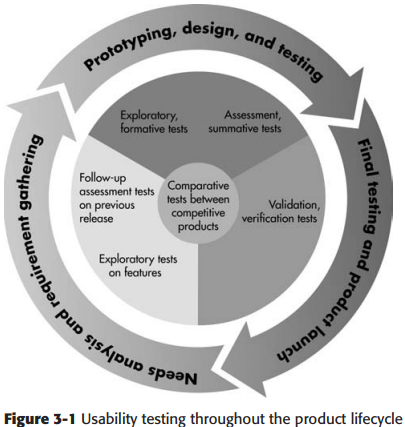
\includegraphics[width=\linewidth]{figures/evaltechcycle.png}

\subsection{Exploratory study}
\begin{itemize}
	\item When / Objective
	\begin{itemize}
		\item Early in development.
		\item Used to examine effectiveness of high-level design aspects, such as: Does the design support user tasks? Does the design communicate the intended workflow properly? 
		\item Used as the foundation of future design work, and is thus important.
	\end{itemize}
	\item Methodology
	\begin{itemize}
		\item Typically conducted using prototypes implementing just what's needed for the test scenario.
		\item Think-aloud testing useful, to gather qualitative data on user thought processes and behavior.
	\end{itemize}
\end{itemize}
\subsection{Assesment / Summative test}
\begin{itemize}
	\item When / Objective
	\begin{itemize}
		\item Early or midways in development, after fundamental design decisions have been made.
		\item Seeks to assess whether the design decisions have been implemented well. Assumes that design decisions are well founded. Looks for specific usability problems while conducting specific tasks
	\end{itemize}
	\item Methodology (compared to exploratory)
	\begin{itemize}
		\item Users perform tasks rather than walking through screens.
		\item Interaction with test moderator is lessened.
		\item Quantitative data will be collected, as the test is about collecting concrete information.
	\end{itemize}
\end{itemize}
\subsection{Validation / Verification test}
\begin{itemize}
	\item When / Objective
	\begin{itemize}
		\item Late in the development cycle.
		\item Compares the product to some specified benchmark or standard. In verification test, verify that previously discovered usability problems have been resolved and that new ones haven't been introduced since. 
		\item Often stated in terms of performance criteria such as efficiency.
		\item Also used to evaluate how the different components in a system work together, that is, validation tests are often integrated tests.
	\end{itemize}
	\item Methodology
	\begin{itemize}
		\item A benchmark is determined beforehand, either in terms of specific error counts or time measures, or simply eliminating earlier problems.
		\item Minimal interaction with test moderator.
		\item High emphasis on quantitative data and how this data is used. 
	\end{itemize}
\end{itemize}


